
\documentclass{beamer}

\usepackage{framed}
\usepackage{graphicx}

\begin{document}
\section{Diverging color palettes}
%====================================%
\begin{frame}[fragile]
\frametitle{Seaborn Workshop}
\large

\noindent \textbf{Diverging color palettes}
\begin{itemize}
\item The third class of color palettes is called “diverging”. These are used for data where both large low and high values are interesting. 
\item There is also usually a well-defined midpoint in the data. 
\item For instance, if you are plotting changes in temperature from some baseline timepoint, it is best to use a diverging colormap to show areas with relative decreases and areas with relative increases.
\end{itemize}
\end{frame}
%====================================%
\begin{frame}[fragile]
	\frametitle{Seaborn Workshop}
	\large
	\begin{itemize}
		\item The rules for choosing good diverging palettes are similar to good sequential palettes, except now you want to have two relatively subtle hue shifts from distinct starting hues that meet in an under-emphasized color at the midpoint. \item It’s also important that the starting values are of similar brightness and saturation.
		\end{itemize}
\end{frame}
%====================================%
\begin{frame}[fragile]
	\frametitle{Seaborn Workshop}
	\large
\begin{itemize}
\item It’s also important to emphasize here that using red and green should be avoided, as a substantial population of potential viewers will be unable to distinguish them.
\item 
It should not surprise you that the \textbf{\textit{Color Brewer}} library comes with a set of well-choosen diverging colormaps.
\end{itemize}

\end{frame}
%====================================%
\begin{frame}[fragile]
\frametitle{Seaborn Workshop}
\large
\begin{verbatim}
sns.palplot(sns.color_palette("BrBG", 7))
\end{verbatim}

\begin{figure}
\centering

\includegraphics[width=0.7\linewidth]{images/color_palettes_54_0}

\end{figure}

\begin{verbatim}
sns.palplot(sns.color_palette("RdBu_r", 7))
\end{verbatim}
\begin{figure}
\centering

\includegraphics[width=0.7\linewidth]{images/color_palettes_55_0}
\end{figure}

\end{frame}
%====================================%
\begin{frame}[fragile]
\frametitle{Seaborn Workshop}
\large


Another good choice that is built into matplotlib is the coolwarm palette. Note that this colormap has less contrast between the middle values and the extremes.
\end{frame}
%====================================%
\begin{frame}[fragile]
	\frametitle{Seaborn Workshop}
	\large
	
\begin{verbatim}
sns.palplot(sns.color_palette("coolwarm", 7))
\end{verbatim}

\begin{figure}
\centering

\includegraphics[width=0.7\linewidth]{images/color_palettes_57_0}
\end{figure}


\end{frame}
%====================================%
\section{Custom diverging palettes with \texttt{diverging\_palette()}}
\begin{frame}[fragile]
\frametitle{Seaborn Workshop}
\large

\begin{itemize}
\item You can also use the seaborn function \texttt{diverging\_palette()} to create a custom colormap for diverging data. (Naturally there is also a companion interactive widget, \texttt{choose\_diverging\_palette()}). This function makes diverging palettes using the husl color system. 
\item You pass it two hues (in degreees) and, optionally, the lightness and saturation values for the extremes. 
\item Using husl means that the extreme values, and the resulting ramps to the midpoint, will be well-balanced

\end{itemize}
\end{frame}
%====================================%
\begin{frame}[fragile]
	\frametitle{Seaborn Workshop}
	\large
	\begin{verbatim}
sns.palplot(sns.diverging_palette(220, 20, n=7))
	\end{verbatim}

\begin{figure}
\centering

\includegraphics[width=0.7\linewidth]{images/color_palettes_59_0}
\end{figure}



\begin{verbatim}
sns.palplot(sns.diverging_palette(145, 280, 
            s=85, l=25, n=7))
\end{verbatim}
	
\begin{figure}
\centering

\includegraphics[width=0.7\linewidth]{images/color_palettes_60_0}
\end{figure}
\end{frame}
%====================================%
\begin{frame}[fragile]
\frametitle{Seaborn Workshop}
\large


The sep argument controls the width of the separation between the two ramps in the middle region of the palette.
\begin{verbatim}
sns.palplot(sns.diverging_palette(10, 220, sep=80, n=7))
\end{verbatim}

\begin{figure}
	\centering
	
\includegraphics[width=0.7\linewidth]{images/color_palettes_62_0}
\end{figure}
\end{frame}
%====================================%
\begin{frame}[fragile]
	\frametitle{Seaborn Workshop}
	\large
It’s also possible to make a palette with the midpoint is dark rather than light.
\begin{verbatim}
sns.palplot(sns.diverging_palette(255, 133, 
     l=60, n=7, center="dark"))
\end{verbatim}

\begin{figure}
	\centering
	
\includegraphics[width=0.7\linewidth]{images/color_palettes_64_0}
\end{figure}

\end{frame}
\section{Changing default palettes with set\_palette()}
%====================================%
\begin{frame}[fragile]
\frametitle{Seaborn Workshop}
\large
\begin{itemize}
\item The \texttt{color\_palette()} function has a companion called \texttt{set\_palette()}. 
\item The relationship between them is similar to the pairs covered in the aesthetics tutorial. 
\item \texttt{set\_palette()} accepts the same arguments as \texttt{color\_palette()}, but it changes the default matplotlib parameters so that the palette is used for all plots.
\end{itemize}

\end{frame}
%====================================%
\begin{frame}[fragile]
	\frametitle{Seaborn Workshop}
	\Large
\begin{framed}
	\begin{verbatim}
def sinplot(flip=1):
  x = np.linspace(0, 14, 100)
  for i in range(1, 7):
      y = np.sin(x + i * .5) * (7 - i)
      plt.plot(x, y * flip)
      sns.set_palette("husl")
      sinplot()
	\end{verbatim}
\end{framed}

\end{frame}
%====================================%
\begin{frame}[fragile]
	\frametitle{Seaborn Workshop}
	\large
	
	
\begin{figure}
\centering
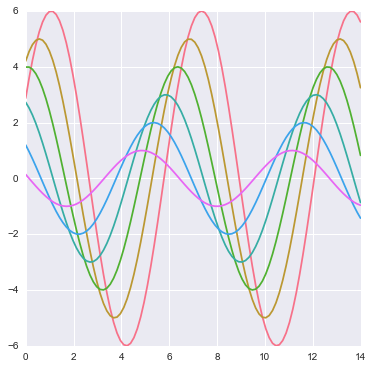
\includegraphics[width=0.7\linewidth]{images/color_palettes_67_0}
\end{figure}

\end{frame}
%====================================%
\begin{frame}[fragile]
	\frametitle{Seaborn Workshop}
	\large
\begin{itemize}
\item The \texttt{color\_palette()} function can also be used in a with statement to temporarily change the color palette.
\end{itemize}
\begin{verbatim}

with sns.color_palette("PuBuGn_d"):
sinplot()
\end{verbatim}

\begin{figure}
	\centering
	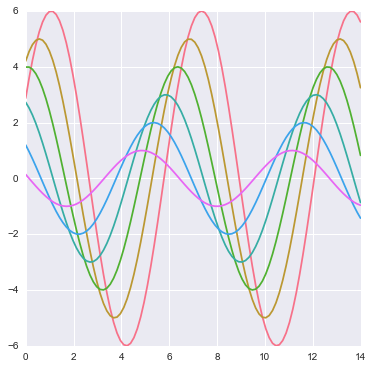
\includegraphics[width=0.7\linewidth]{images/color_palettes_67_0}
\end{figure}.png
\end{frame}
%====================================%

\end{document}